\section{嵌套虚拟化（二）：HyperTurtle 与跨层往返的削减}\label{sec:hyperturtle}

计算机领域有一句话：一件事如果复杂到不好直接描述，就不妨在中间加一层抽象。虚拟化本身就是这句话的产物——VMM 把整台机器的指令集、地址空间、中断与设备重新表述成一组虚拟接口，于是“在一台机器上跑多台机器”不再需要逐条处理每个细节，而变成对这套接口的一次实现。嵌套虚拟化是把同一层抽象再叠一次：L1 拿到的不是真实机器，而是一套虚拟的虚拟化接口，它用这套接口去管理 L2。

抽象层不是免费的。每穿过一次接口边界都要付出模式切换、状态翻译与事件转发的代价，叠了两层，这条路径就要走两遍。跨抽象层的性能优化由此成为一个独立的问题：目标不是取消抽象——那会连带丢掉隔离与管理权——而是让一部分操作不必真的穿过它，在保持接口语义的前提下把执行留在更靠底的那一层。HyperTurtle 正落在这个位置上：L1 hypervisor 通过 eBPF 把自身的处理逻辑注册成 L0 事件处理路径上的 hook，L2 触发相应事件时由 L0 就地调用这段程序完成处理，省掉进入 L1 的那次往返，而策略仍由 L1 定义~\cite{source8}。

上一章已经用普通嵌套的九步路径说明：当 $EPT_{0\to2}$ 与 $EPT_{1\to2}$ 都缺项时，L0 要先进入 L1 补蓝本，再让 L2 重执行、再次退出，最后才能补硬件实际使用的影子表。本章不再并列展开网络、采样和 artifact 程序，而是只沿这一次 $EPT_{0\to2}$ page fault 往下走：先分清两张 EPT 各自缺什么，再看 hyperupcall 如何借助 L1 中 QEMU 的页表和预分配帧池补 $EPT_{1\to2}$，最后分析 L0 如何收尾、L1 如何同步，以及何时必须回退。

图~\ref{fig:ht-worldswitch} 给出这一改法的总览：左栏普通嵌套把 L2 的事件经 L0 转发给 L1 hypervisor，右栏则由 L0 在处理路径上直接执行 hyperupcall。它强调的是处理位置的变化；本章随后补全图中略去的两张 EPT、QEMU 页表与回退条件。

\begin{figure}[htbp]
\centering
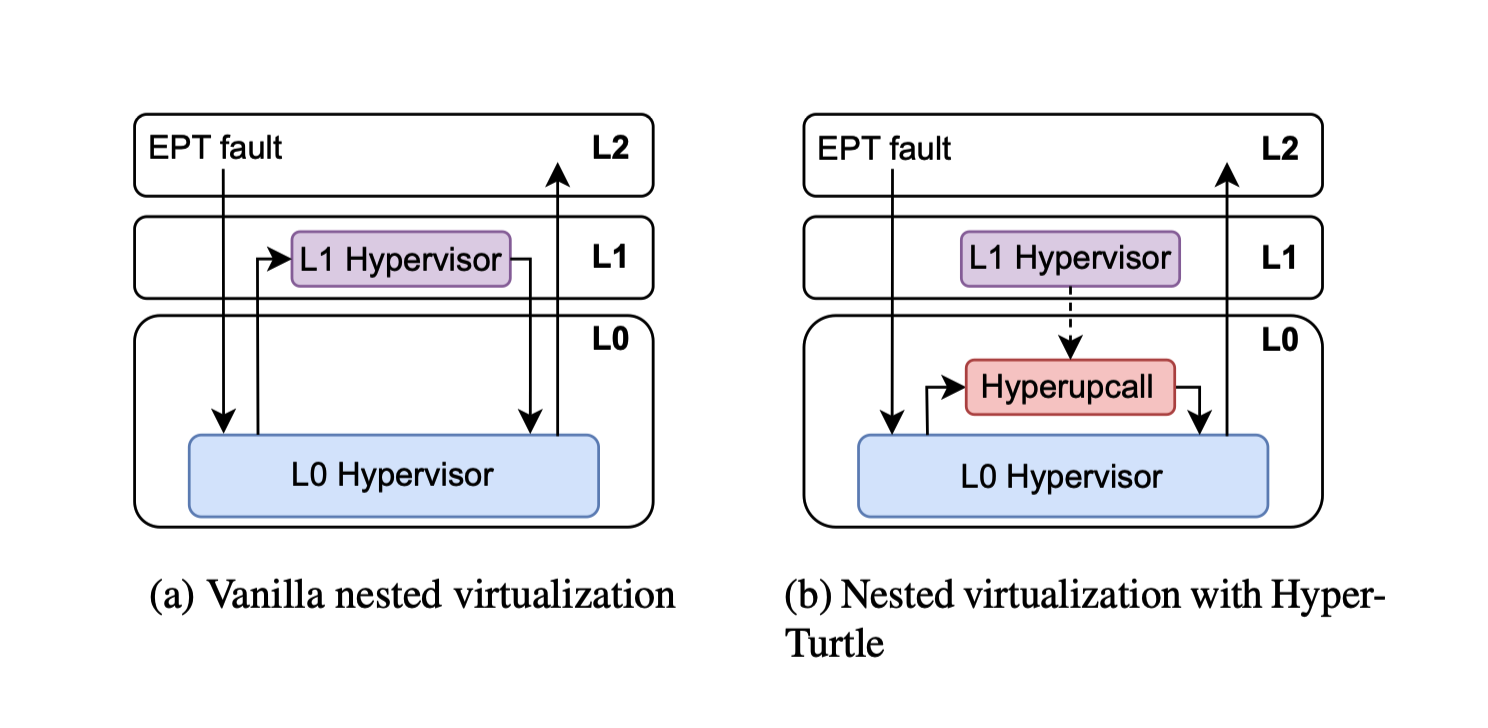
\includegraphics[width=0.98\linewidth]{figures/hyperturtle-fig1.png}
\caption[嵌套虚拟化中的 world-switch 问题]{嵌套虚拟化中的 world-switch 问题。(a) 普通嵌套：L2 的 EPT fault 由 L1 hypervisor 处理，L0 转发该事件并增加跨层切换；(b) HyperTurtle：L0 通过 hyperupcall 就地执行下放的 eBPF 处理逻辑。引自 Ben Zur et al., USENIX ATC 2025, Figure 1~\cite{source8}。}
\label{fig:ht-worldswitch}
\end{figure}

\subsection{从两张 EPT 缺项定位问题}\label{sec:ht-motiv}

L2 中的一次普通访存先由 L2 页表把 L2 虚拟地址翻译成 L2 物理地址（L2-PA），再由硬件当前装载的 $EPT_{0\to2}$ 把 L2-PA 翻译成 L0 物理地址（L0-PA）。后一跳缺项会触发 EPT violation，CPU 从 L2 退出到 L0，原访存指令尚未完成。L0 此时面对的不是一个孤立的“缺页”请求，而是两个必须分别回答的问题：L1 是否已经为这段 L2 内存分配了 L1 物理帧，以及 L0 是否已经把这个结果拼进 $EPT_{0\to2}$。

为区分这两件事，记发生 fault 的 L2-PA 为 $P$，承载它的 L1 物理帧地址为 $M$，最终机器物理地址为 $H$。两张表与 L0 自有的 $EPT_{0\to1}$ 形成如下关系：

\begin{equation}
EPT_{1\to2}:P\rightarrow M,\qquad
EPT_{0\to1}:M\rightarrow H,\qquad
EPT_{0\to2}:P\rightarrow H.
\end{equation}

其中 $EPT_{1\to2}$ 是 L1 KVM 为 L2 维护的蓝本，$EPT_{0\to1}$ 描述 L1 自身内存到真实机器内存的映射，$EPT_{0\to2}$ 则是 L0 为运行 L2 而合成的影子表。HyperTurtle 的 hook 不在每次 $EPT_{0\to2}$ 缺项时都接管，而是放在 L0 检查蓝本之后：只有 $EPT_{1\to2}$ 也为 non-present 时，才需要替代原本进入 L1 的那一段处理~\cite{source8}。

\begin{lstlisting}[style=pseudopy,caption={L0 对一次 L2 EPT fault 的缺项分流（逻辑伪代码）},label={lst:ht-dispatch}]
def handle_l2_ept_fault(P, access_type):
    # CPU 已从 L2 退出；P 是 L2-PA，指令尚未完成
    if ept12_lookup(P).present:
        # L1 已分配 L1 帧，L0 只需合成影子表项
        install_ept02_from_ept12(P)
        resume_l2()
        return

    # EPT12 也缺项：传统路径在这里把 fault 注入 L1
    if hyperupcall_ept_fault(P, access_type) == SUCCESS:
        install_ept02_from_ept12(P)  # hyperupcall 已补好蓝本
        resume_l2()                  # 不进入 L1
    else:
        inject_ept_fault_to_l1(P, access_type)
        resume_l1()                  # 保留原有慢路径
\end{lstlisting}

代码块~\ref{lst:ht-dispatch} 的第一条分支说明，$EPT_{0\to2}$ 缺项本身不等于 hyperupcall 必须工作；蓝本已有映射时，L0 直接补影子表即可。后一条分支才是本章的主线：hyperupcall 的任务是补 $EPT_{1\to2}$，不是替 L0 直接写 $EPT_{0\to2}$。它返回成功后，L0 仍按原有规则完成 $P\rightarrow M\rightarrow H$ 的合成，再恢复 L2。

普通嵌套下，这个“蓝本也缺”的情形造成六次 world-switch：L2 首次退出、L0 进入 L1、L1 恢复动作陷入 L0、L0 进入 L2、L2 重执行后再次退出、L0 最终恢复 L2。HyperTurtle 成功时把路径压成 $L2\rightarrow L0\rightarrow L2$：省掉的是进入 L1 建蓝本、L1 的恢复尝试，以及 L2 第一次重执行后的第二次 fault；L0 对影子表的建立并未被取消~\cite{source8}。

\subsection{hyperupcall 的注册与状态准备}\label{sec:hyperturtle-design}

HyperTurtle 把 L1 定义的这段建表逻辑写成 eBPF 程序，称为 hyperupcall。安装与执行必须分开理解：安装时，L1 通过 hypercall 把编译后的程序交给 L0，经 L0 的 KVM 与用户态安装组件完成验证和加载，再把程序链接到 L0 的 EPT fault hook。加载与链接拆成两个 hypercall，使同一程序可以挂到多个 hook 而不必重复加载。完成安装后，程序不再经 hypercall 调用，而是由 L0 在处理 L2 事件时直接触发~\cite{source8}。

这段程序不能任意读写 L1。新增 helper \code{bpf_probe_read_hyperupcall} 只允许它读取有效、已映射且属于其所属 L1 的物理内存；eBPF verifier 检查程序自身的内存访问、循环等约束，VM 归属与 helper 的地址检查再限定它能看哪一份 guest 状态。L0 与 L1 之间还通过共享的数组型 eBPF map 交换数据，map 经共享内存 PCI 设备映射到 L1，因而双方可以并发访问同一份状态，而不是每次借 VM-exit 传递消息~\cite{source8}。

EPT 案例需要预先准备四类共享状态：L1 维护的预分配帧池、QEMU 进程的页表根 \code{cr3}、记录 hyperupcall 所建映射的 fault log，以及记录 L1 侧 shmem 缺页的 page fault log；另有一把双方都能获取的共享锁。eBPF 上下文不适合完成复杂的内存分配，所以帧池由 L1 异步补充，或在其因 VM-exit 获得处理机会时批量补充。论文实验采用 4096 帧的池，以避免同步补充；池空不是错误，而是回退条件~\cite{source8}。

\subsection{沿一次 EPT fault 展开 HyperTurtle}\label{sec:nested-ht-ept}

本例采用论文限定的 shmem 文件后备内存：L1 中的 QEMU 通过 \code{mmap} 获得一段自己的虚拟内存，再把它注册为 L2 的 guest RAM。为叙述具体，以下直接称这一 VMM 为 QEMU；Cloud Hypervisor 在该路径中承担相同角色。论文原型面向 QEMU、Cloud Hypervisor 与 Kata Containers 所采用的这类后备方式，不能把结论直接推广到任意内存后端~\cite{source8}。

\subsubsection{先分清 QEMU 页表与 EPT}\label{sec:ht-qemu-pagetable}

QEMU 虽然管理 L2，本身仍是 L1 中的一个用户态进程。它访问自己的代码、堆和所映射的 L2 内存时，使用 L1 内核为其维护的普通进程页表：

\begin{equation}
\text{QEMU 的 L1-VA }V
\xrightarrow{\text{QEMU 页表}}\text{L1-PA }M.
\end{equation}

这里的“QEMU 页表”就是前面所说的 VMM 页表，不是 EPT，也不是 L2 中某个进程的页表。其根地址保存在 QEMU 进程的 \code{cr3} 中。QEMU 把一段起始虚拟地址为 $V_{\text{base}}$ 的内存注册成起始 L2-PA 为 $P_{\text{base}}$ 的内存槽后，同一页便有两个不同的名字：L2 看到 $P$，QEMU 看到 $V$。二者数值不必相等，逻辑位置由下式对应：

\begin{equation}
V=V_{\text{base}}+(P-P_{\text{base}}).
\end{equation}

QEMU 页表负责 $V\rightarrow M$，$EPT_{1\to2}$ 负责 $P\rightarrow M$。两棵树的根指针、输入地址空间和维护者都不同，不存在一方包含另一方的关系；它们只是可以在输出端指向同一个 L1 物理帧。L2 运行时使用 EPT，QEMU 自己访问该页时使用普通页表。HyperTurtle 读取 QEMU 页表，正是为了检查这页是否已经有一个可复用的 $M$。

\subsubsection{在 L0 内补全 L1 的蓝本}\label{sec:ht-upcall-body}

现在回到代码块~\ref{lst:ht-dispatch} 中调用 hyperupcall 的路径。L0 发现 $EPT_{1\to2}[P]$ 为 non-present 后，调用 hyperupcall，并传入 $P$ 与读写类型。程序首先尝试获取共享锁；成功后才检查 QEMU 页表、并发日志和帧池。整个快路径可概括为代码块~\ref{lst:ht-ept-body}。

\begin{lstlisting}[style=pseudopy,caption={hyperupcall 为缺失的蓝本寻找 L1 物理帧（逻辑伪代码）},label={lst:ht-ept-body}]
def hyperupcall_ept_fault(P, access_type):
    if not try_lock(shared_ept_lock):
        return FALLBACK
    if hyperupcall_fault_log.is_full():
        unlock(shared_ept_lock)
        return FALLBACK

    # 由内存槽的位置对应，算出 QEMU 看到的虚拟地址
    V = qemu_userspace_base(P) + (P - qemu_guest_phys_base(P))

    # 路径一：QEMU 已有 V -> M，复用这页，不再分配帧
    M = walk_qemu_page_table(shared_qemu_cr3, V)
    if M is not None:
        ept12_install(P, M, access_type)
        hyperupcall_fault_log.append(P)
        unlock(shared_ept_lock)
        return SUCCESS

    # QEMU 页表也没有：先看 L1 侧是否正在处理同一页
    if page_fault_log.contains(P):
        unlock(shared_ept_lock)
        return FALLBACK

    # 路径二：消费 L1 预分配的帧，补 EPT12 并通知 L1
    M = frame_pool.pop()
    if M is None:
        unlock(shared_ept_lock)
        return FALLBACK

    ept12_install(P, M, access_type)
    hyperupcall_fault_log.append(P)
    unlock(shared_ept_lock)
    return SUCCESS
\end{lstlisting}

遍历 QEMU 页表时，hyperupcall 并不把 QEMU 的 \code{cr3} 装入当前 CPU，也不切换到 QEMU 地址空间。它只是把共享的 \code{cr3} 当作页表根指针，使用受限 helper 逐级读取 QEMU 的普通页表项。若查到 $V\rightarrow M$，说明 QEMU 已经为这页建立好 L1 侧映射，程序可以直接构造 $EPT_{1\to2}:P\rightarrow M$，无需消耗帧池。

若 QEMU 页表也缺项，程序还不能立即分配，因为 L1 的 shmem 缺页路径或 \code{virtiofsd} 可能正在处理同一页。page fault log 用来暴露这类并发活动；若其中已有 $P$，hyperupcall 放弃快路径，由 L1 沿原有逻辑完成处理。只有没有并发冲突时，程序才从帧池取出 $M$，写入 $EPT_{1\to2}$，并把 $P$ 追加到 hyperupcall fault log。帧池耗尽、日志写满、取锁失败或遇到不支持的情况，都返回回退而不是在 L0 中勉强完成~\cite{source8}。

无论映射来自 QEMU 页表还是帧池，hyperupcall 返回成功时改变的都只是蓝本及共享日志。随后 L0 重新取得 $P\rightarrow M$，经 $EPT_{0\to1}$ 得到 $M\rightarrow H$，建立 $EPT_{0\to2}:P\rightarrow H$，恢复 L2。L2 重执行原访存指令，这一次第二级翻译已经齐全，不再需要为同一缺项第二次退出。

\subsubsection{恢复 L2 之后，L1 仍须同步}\label{sec:ht-ept-sync}

快路径结束于 L2，并不意味着 L1 的所有状态已经同步。尤其是从帧池取页时，$EPT_{1\to2}$ 已有 $P\rightarrow M$，QEMU 页表却可能仍没有对应的 $V\rightarrow M$。若让这种状态无限期滞留，QEMU 与其他共享该文件后备内存的组件就可能看到不一致的映射。HyperTurtle 因而把“让 L2 立即继续运行”与“把变化补记到 L1”拆成两个阶段。

代码块~\ref{lst:ht-ept-sync} 的两个函数有不同的触发者。第一个由 L1 KVM 在下一次因 VM-exit 进入 L1 时执行，用来消费 hyperupcall 留下的 fault log。第二个则是对 L1 原有 shmem page-fault handler 的包装：当 L1 中的 QEMU 或 \code{virtiofsd} 等文件后备内存使用者访问一个尚未在自身地址空间建立映射的 shmem 页，因而触发 L1 的普通页故障时，L1 内核进入这个包装函数。它不是 L2 发生 EPT fault 时由 L0 调用的 hyperupcall；前者处理 L1 进程地址空间的缺页，后者处理 L2 第二级地址翻译的缺项。

\begin{lstlisting}[style=pseudopy,caption={L1 后续补偿与 shmem 缺页路径的同步（逻辑伪代码）},label={lst:ht-ept-sync}]
def l1_on_next_vmexit():
    for P in hyperupcall_fault_log.drain():
        V = qemu_va_for_l2_pa(P)
        fault_qemu_va_into_address_space(V)  # 补 QEMU 页表等 L1 状态

def wrapped_l1_shmem_fault(P):
    spin_lock(shared_ept_lock)
    if ept12_lookup(P).present:
        map_existing_ept12_page_to_l1(P)  # hyperupcall 已先建映射
    original_shmem_fault_handler()
    page_fault_log.append(P)              # 告知 L0 侧程序：L1 处理过此页
    unlock(shared_ept_lock)
\end{lstlisting}

代码块~\ref{lst:ht-ept-sync} 的两个函数有不同触发者，此处分别说明。第一个由 L1 KVM 在下一次因 VM-exit 进入 L1 时执行，消费 hyperupcall fault log，并把其中 L2-PA 对应的 L1-VA fault 进 QEMU 地址空间。第二个则是对 L1 原有 shmem page-fault handler 的包装：当 L1 中的 QEMU 或 \code{virtiofsd} 等文件后备内存使用者访问一个尚未在自身地址空间建立映射的 shmem 页，因而触发 L1 的普通页故障时，L1 内核进入这个包装函数。它不是 L2 发生 EPT fault 时由 L0 调用的 hyperupcall；前者处理 L1 进程地址空间的缺页，后者处理 L2 第二级地址翻译的缺项。包装函数先取得同一把锁，再检查 $EPT_{1\to2}$ 是否已被 hyperupcall 填好；若已填好就复用该映射，随后执行原处理并记录 page fault log。这样，即使尚未发生一次进入 L1 的退出，L1 侧也不会忽略 L0 已经建立的映射~\cite{source8}。

这组机制也限定了 HyperTurtle 的实际贡献。它不是把 L1 从内存管理中删除，而是把 L2 继续运行所必需的蓝本建立留在 L0，把 L1 可见状态的补偿经日志延后；锁与双日志承担并发一致性，帧池承担资源供给，原 L1 路径承担所有快路径不适用的情况。优化的核心不是“eBPF 本身更快”，而是把一次跨层操作改造成一个有共享状态协议的就地处理路径。

\subsection{实验证据与适用边界}\label{sec:ht-eval}

上述机制的收益应当用同一条 EPT 路径衡量，而不能把不同子系统的加速比合并成“系统加速”。论文在 Kata 虚拟机内触发 1\,GiB 内存的按需映射，报告 HyperTurtle 相对普通嵌套 L2 的 EPT fault 平均延迟改善约 $5.25\times$、99p 延迟改善约 $4.76\times$；平均延迟接近其非嵌套参考，99p 则仍有约 8\% 差距~\cite[\S5.1]{source8}。这些数字支持的是“适用缺页热路径的往返显著减少”，不是任意访存都获得同样加速。

端到端意义来自 Kata 服务启动实验：论文从发出启动命令计时至容器内 Web 服务能够响应请求，而非只测 guest 内核 boot。不同镜像下，4\,KiB 页配置的平均启动时间缩短 27\%，2\,MiB 页配置为 8\%。大页情形仍有部分路径以 4\,KiB 页映射 L2 内核，因此优化并未完全失去作用，但收益较小~\cite[\S5.2]{source8}。这组结果说明收益依赖缺页在负载中的占比、页大小与后备内存组织；对已经建立好映射的稳定运行阶段，不能由启动结果外推同样的提升。

实验平台与配置也构成结论边界。论文使用双路 Xeon Silver 4216，固定 vCPU 与 vhost 线程在同一 NUMA 节点内的不同物理核，关闭 SMT，并设置 \codeplain{idle=poll} 与 \codeplain{nopti}。这些条件会影响空闲等待与隔离成本，因此本文只把数值视为论文报告，不将其当作生产环境的预先保证~\cite[\S5, Table 6]{source8}。

原型本身的限制更直接：EPT hyperupcall 不支持分配大页，对尚未映射进 QEMU 页表的部分 page-cache 页面不能直接处理，且全局 EPT hook 暂时只允许一个 L1 为一个 L2 使用该处理器。复杂 L1 功能的并发同步也限制了完整下放，所以原有 L1 路径必须长期保留~\cite[\S4.8]{source8}。后续评测若只继续降低理想路径延迟，仍不足以回答其可部署性；还应控制帧池补充频率、日志占用率和锁竞争，报告回退率、尾延迟及宿主 CPU 时间，检验省下的切换是否被一致性维护重新消耗。

安全边界同样需要与性能分开评价。verifier 约束的是程序执行形态，helper 的地址授权、VM 归属检查、日志协议与锁才决定它实际能访问和修改什么。该机制假定 L0 能读取并处理 L1 的相关状态，不能直接套用到把 L0 排除出信任边界的机密虚拟机模型。沿着本例可以得到一个更准确的总结：HyperTurtle 没有消除 $EPT_{0\to2}$ fault，也没有取代 L1 的内存管理；它把两张表都缺项时原本必须进入 L1 的一段工作，改为 L0 内可验证、可回退且带事后同步的处理，从而保留多层语义而缩短其关键路径。
